\documentclass[reprint,nofootinbib]{revtex4-2}
\usepackage[dvipsnames]{xcolor}
\usepackage{tikz}
\usepackage{amsthm,amsmath,amssymb}
\usetikzlibrary{arrows.meta}
\usetikzlibrary{positioning,fit,backgrounds}
\usetikzlibrary{decorations.pathmorphing,patterns}
\usepackage{tikz}
\usepackage{tikz-network}

\begin{document}

   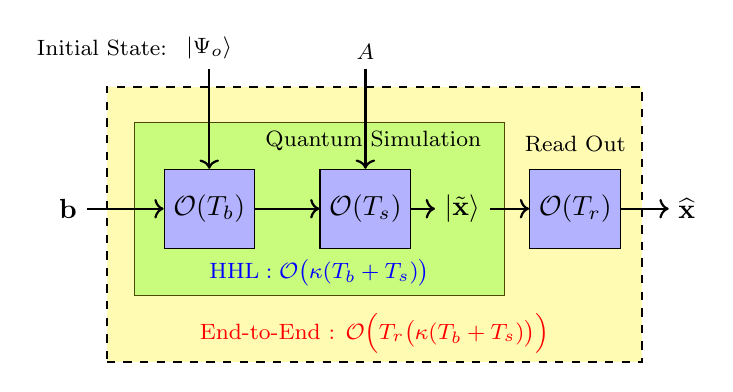
\begin{tikzpicture}
    % Outer box
    \node [draw, rectangle, minimum width=4.7cm, minimum height=2.2cm,fill=green!30] (p) at (0,0) {};
      \node [draw, dashed,thick,rectangle, minimum width=6.8cm, minimum height=3.5cm,fill=yellow,fill opacity=0.3] (p1) at (0.7,-0.2) {};
    \node [left=6mm of p] (in) {$\mathbf{b}$};
    % Left inner box
    \node [draw, rectangle, minimum width=1cm, minimum height=1cm, align=center,fill=blue!30] (b) at (-1.4,0) {$\mathcal{O}(T_b)$};
      \node [above=0.5in of b] (b1) {\footnotesize \textcolor{black}{$|\Psi_o\rangle$}};
       \node [left=0mm of b1] (b2) {\footnotesize \textcolor{black}{Initial State:}};
    % Right inner box
    \node [draw, rectangle, minimum width=1cm, minimum height=1cm, align=center, right=1mm of b,fill=blue!30] (A) at (-0.1,0) {$\mathcal{O}(T_s)$};
      \node [right=3mm of A] (out) {$|\Tilde{{\mathbf{x}}}\rangle$};
       \node [above=1mm of A,xshift=1mm] (A1)  {\footnotesize \textcolor{black}{Quantum Simulation}};
       \node [above=0.5in of A] (a1) {\footnotesize \textcolor{black}{$A$}};
      \node [draw, rectangle, minimum width=1cm, minimum height=1cm, align=center, right=5mm of out,fill=blue!30] (R){$\mathcal{O}(T_r)$};
        \node [above=1mmof R] (R1) {\footnotesize \textcolor{black}{Read Out}};
         \node [right=6mmof R] (R2) {$\widehat{\mathbf{x}}$};
       \node [above=0.01mm of p.south] (A2) {\footnotesize \textcolor{blue}{$\text{HHL}: \mathcal{O}\big(\kappa(T_b+T_s)\big)$}};
     \node [above=0mm of p1.south] (o) {\footnotesize \textcolor{red}{End-to-End : $\mathcal{O}\Big(T_r\big(\kappa(T_b+T_s)\big)\Big)$}};
    % Arrow from outer box to left inner box
    \draw [->,thick] (in) -- (b.west);
    \draw [->,thick] (b.east) -- (A.west);
    \draw [->,thick] (A.east) -- (out);
   \draw [->,thick] (out.east) -- (R);
   \draw [->,thick] (R.east) -- (R2);
    \draw [<-,thick] (b.north) -- (b1);
    \draw [<-,thick] (A.north) -- (a1);
\end{tikzpicture}

\end{document}